%!TEX root = ../../../super_main.tex
\section{Settings Alignment}
\label{sec:settings_alignment}

The settings tab in the \launcher contains the different settings for the user. We noticed during the development, that some of the settings in the panel are not aligned, which gives a bad user impression. We are able to confirm in the code, that the misplacement of the settings is caused by the way a \androidinline{SwitchPreference} is made in Android. By default a \androidinline{SwitchPreference} contains a picture to the left, then some text, and then a switch. As a result, the text is moved to the right to accommodate for the fact that a picture can be present. We intend to change it so that all the settings in the settings panel are aligned to the left side, such that the panel has a consistent and smooth look. The look of the panel with misplaced settings can be seen in \figref{fig:settings_alignment_bad}.

\begin{figure}[!htbp]
    \centering
    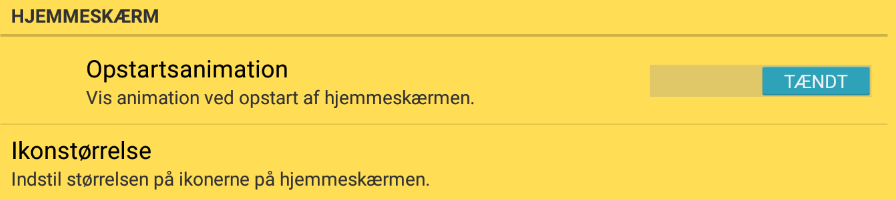
\includegraphics[width=\textwidth]{sprint_one/settings_alignment/bad_alignment}
    \caption{Unaligned settings}
    \label{fig:settings_alignment_bad}
\end{figure}

\subsection{Solution} 
\label{sub:settings_alignment_solution}
We do not want to use pictures as an indicator for our SwitchPreference, so we create our own \androidinline{SwitchPreference} subclass. This allows us to change the visibility of the hidden picture to be ``GONE'' instead. With the picture being gone, the text is able to use the space otherwise reserved for the picture, and nicely align with the settings below it. The panel with properly aligned settings can be seen in \figref{fig:settings_alignment_good}

\begin{figure}[!htbp]
    \centering
    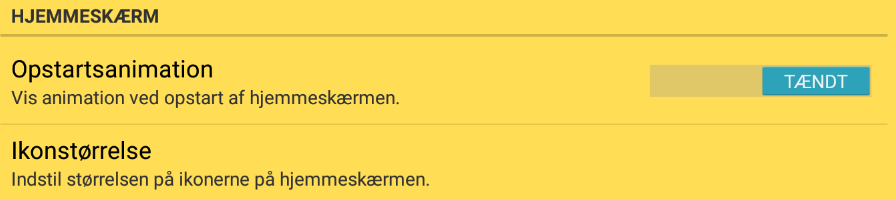
\includegraphics[width=\textwidth]{sprint_one/settings_alignment/good_alignment}
    \caption{Aligned settings}
    \label{fig:settings_alignment_good}
\end{figure}